


\section{Experiment 1}

In Experiment 1, participants completed
a mouse tracking version of \citegap{Gelman1986}{'s} triad task,
with natural categories.
In the original version of this task, children had to choose
between generalising a property from a base species
to another conceptually-related species,
or to an unrelated but perceptually similar one.
This experiment is, to my knowledge,
the first to include a control condition,
in which both perceptual and conceptual information cue the same response.
Using this experimental manipulation, it is possible to
explore the role these perceptual cues play in reasoning.
Additionally, by recording participants' mouse cursor movements,
the experiment provides a window into processes during reasoning,
rather than just the final inferences participants make.



\subsection{Method}

\subsubsection{Participants}

Fifty nine undergraduate students took part in exchange for course credit.

\subsubsection{Stimuli \& Procedure}

At  the start of the experiment,
participants were presented with a framing story,
based on those used by \citet{Sloutsky2007} and \citet{Gelman2013c}.
This introduced a boy, Mark, who had moved to a country called Elbee,
where his teacher was teaching him
about the plants and animals found there.
They were instructed that they would be told
some of the facts that Mark's teacher had told him,
and shown pictures of three animals.
They were also instructed that their task was to decide,
given a fact about one species,
which of the two other species
this fact was likely to be true for.
This was illustrated using an example.

Participants then completed ten induction trials, in random order.
Induction stimuli were similar to those used by \citet{Gelman1986},
but were created for the current experiment.
They consisted of ten sets of species of plants and animals.
The full set of stimuli used can be found in Appendix~\ref{appendix:exp1_stimuli}.
Each set was made up of a \emph{base} species,
a \emph{correct response} species belonging to
the same super-ordinate category as the base,
and two \emph{foil} species, belonging to a different category:
one that was intended to be
perceptually similar to the base, and one that was not.
Each species was represented in the experiment
by a colour photograph (see Figure~\ref{fig:exp1-screenshot1},
and Appendix~\ref{appendix:exp1_stimuli}).
For each participant, five stimuli sets were randomly chosen as
conflict trials, and presented with the foil
that was perceptually similar to the base.
The remaining sets were designated control trials
and presented with the foil dissimilar to the base.

On each trial, the base was presented
in the centre of the screen,
with a property of that species shown above the image.
Blank genetic properties were used, of the form
``This one has gene 4ew. What else do you think has gene 4ew?''.
After clicking a button marked ``NEXT'' in the bottom centre of the screen,
images of the two possible response species
appeared in the top left and right corners,
with their positions randomised on each trial
(Figure~\ref{fig:exp1-screenshot1}).
Participants responded by clicking on one or other image,
and the position of the mouse cursor was recorded as they did so.

\begin{figure}[pt]
  \centering
  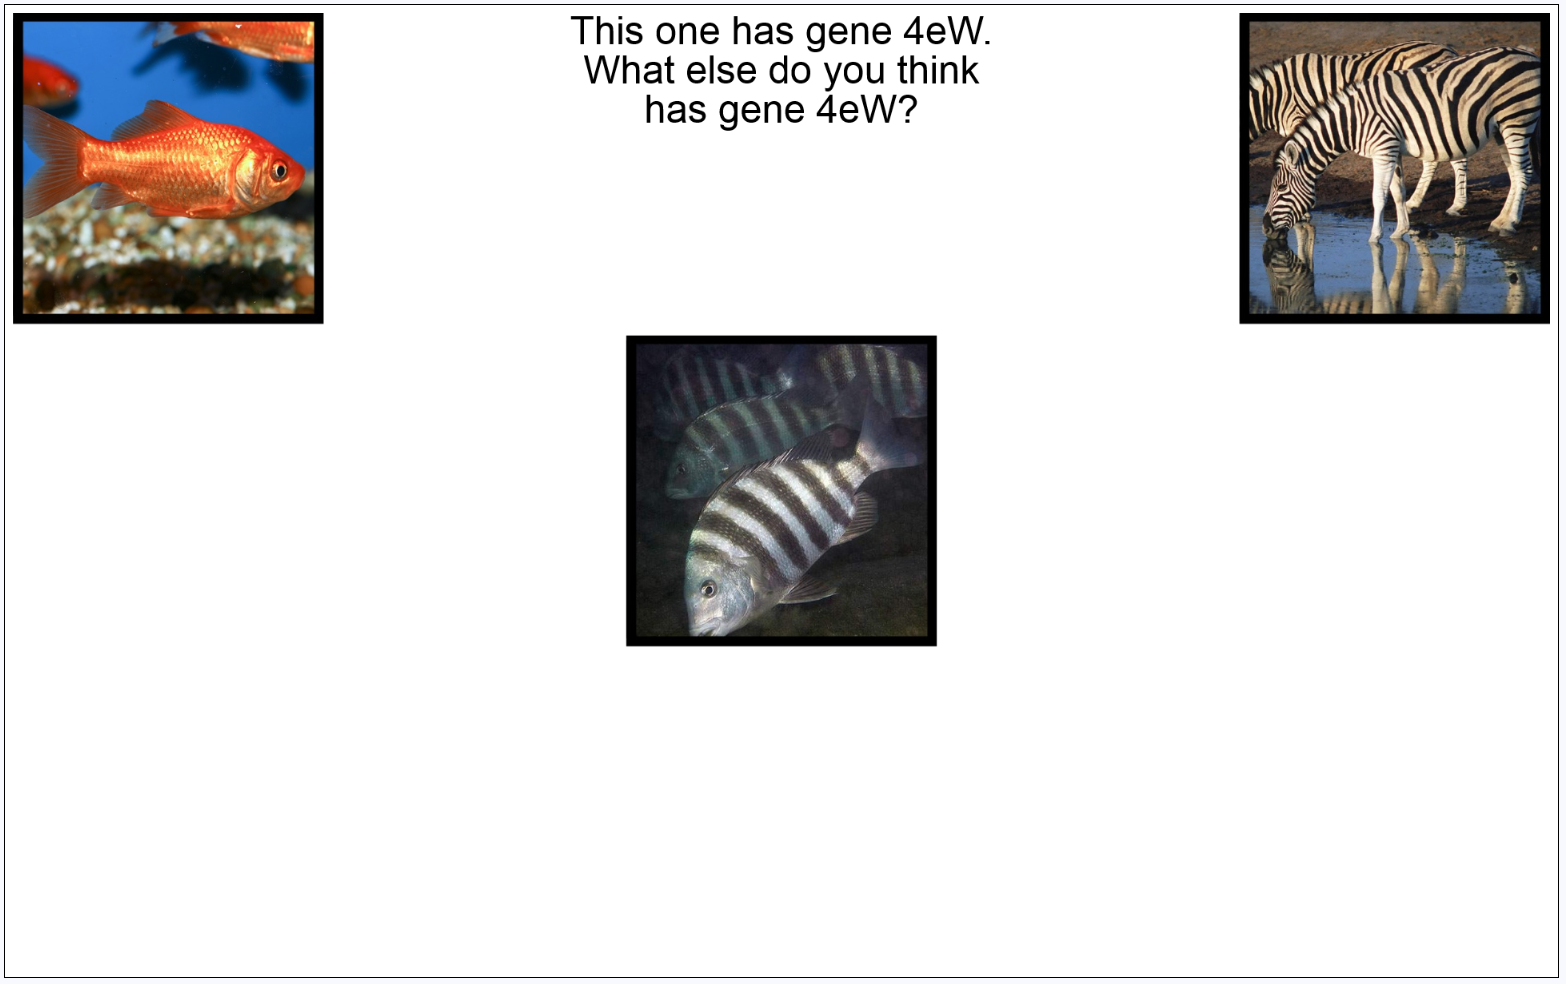
\includegraphics[width=.8\textwidth]{imgs/natural_conflict.png}
  \caption[Screen shot of conflict trial from Experiment 1.]{
    Screen shot of conflict trial from Experiment 1.
    The base image, a striped fish, belongs to the same category as the
    correct response option, the goldfish shown in the top left,
    but is perceptually similar to the foil option,
    the zebra in the top right.}
  \label{fig:exp1-screenshot1}
\end{figure}

\begin{figure}[pb]
  \centering
  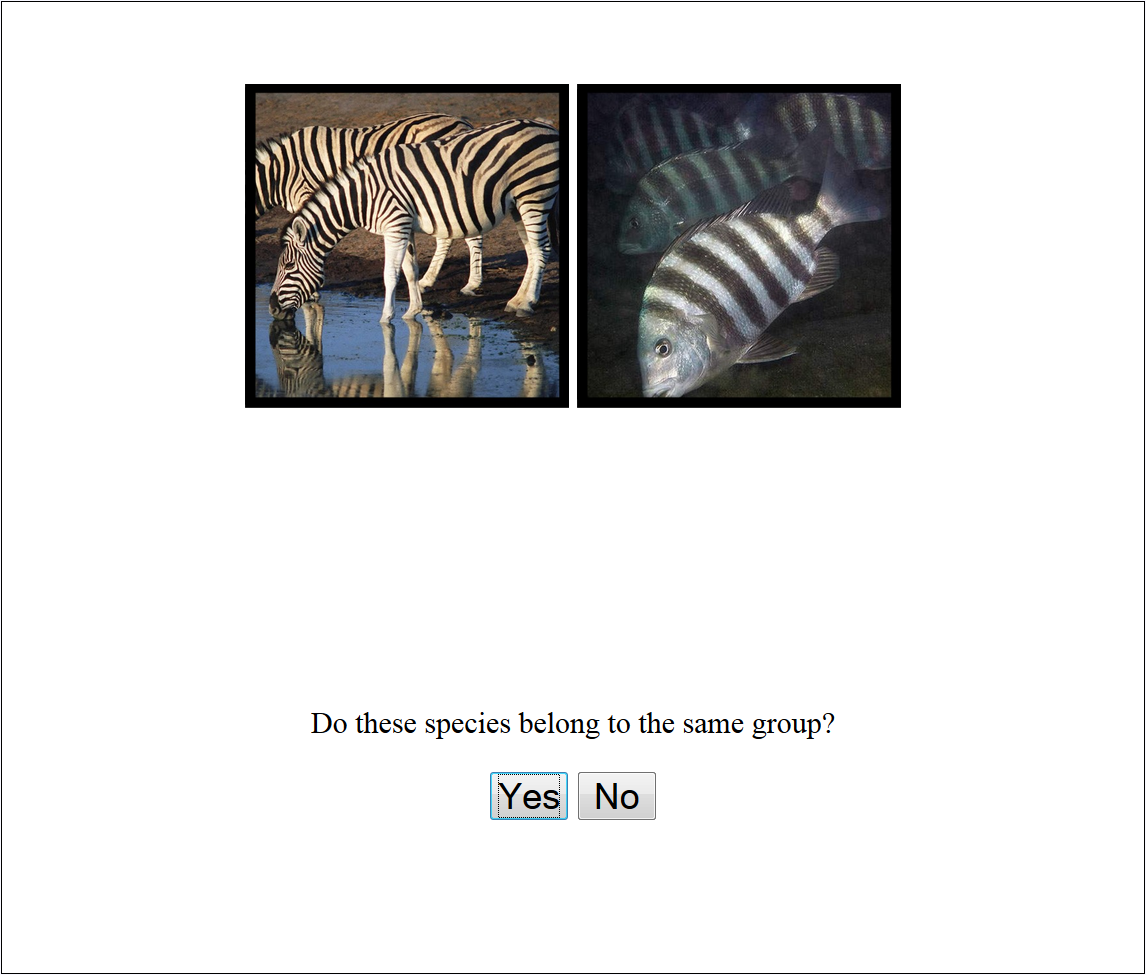
\includegraphics[width=.7\textwidth]{imgs/exp1_posttest.png}
  \caption{Screen shot from the post-test check, Experiment 1.
    \label{fig:exp1-screenshot2}}
\end{figure}


After the reasoning trials, participants completed a post-test check.
This was to ensure that participants possessed the appropriate
structured knowledge about the relationships between
the species used.
Each base species was presented twice,
once alongside its corresponding correct response,
which belonged to the same biological category,
and once alongside its perceptually similar foil,
which did not.
The left-right positioning of these images
was randomised for each trial.
Participants were instructed to indicate
if each pair of species belonged to the same biological group.
% (Figure~\ref{fig:exp1-screenshot2})
The order of presentation of the post-test stimuli was totally randomised.
